\subsection{Depth Sensors}

Depth sensors play an increasingly important role in modern robotic applications.
They give a robot a fast mean to detect obstacles and locate itself in its environment.
The following paragraphs describe the underlying sensing principles\cite{blais_2003} for the depth sensors commonly used in mobile robotic applications.

\subsubsection{Structured-Light Depth Sensors}

\begin{figure}[H]
    \centering
    \begin{subfigure}[t]{0.45\textwidth}
        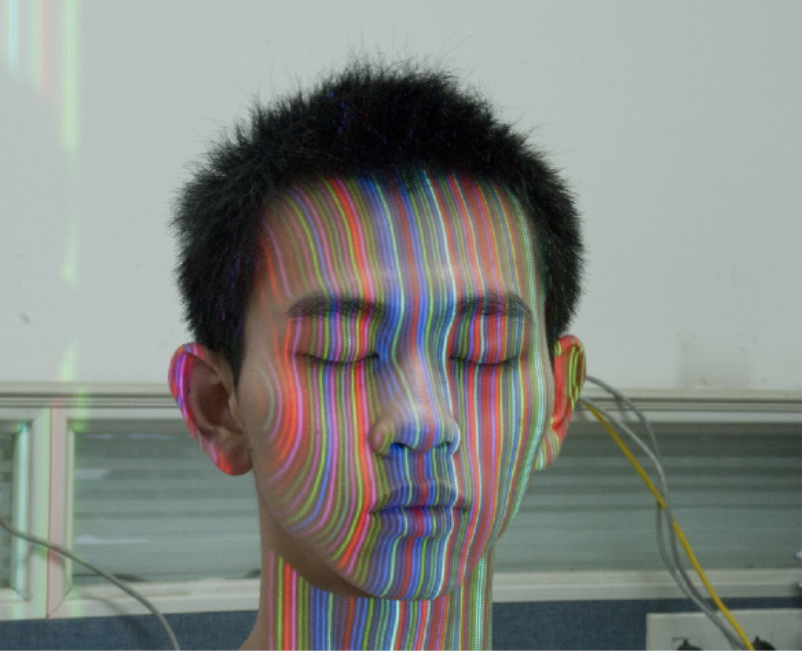
\includegraphics[width=\textwidth]{chapter03/img/depth_pattern_face.png}
        \caption{Visible structured light pattern}
    \end{subfigure}
    \begin{subfigure}[t]{0.45\textwidth}
        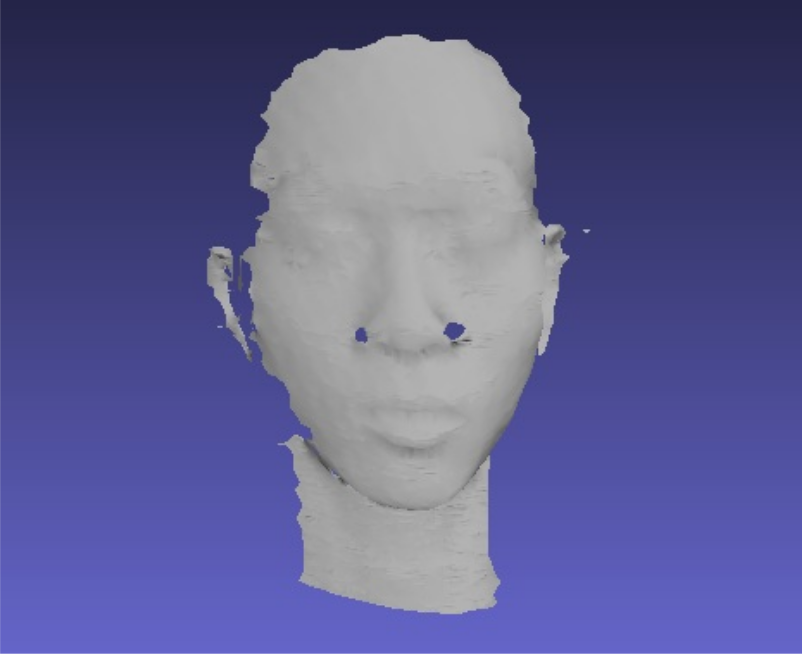
\includegraphics[width=\textwidth]{chapter03/img/depth_face_reconstructed.png}
        \caption{Reconstructed result}
    \end{subfigure}
    \caption[Demonstration of structured-light depth sensors]{\emph{Demonstration of structured-light depth sensors.} One way to reconstruct depth information are structured light depth sensors. A predefined light pattern is projected into space. As the photons reflect from obstacles at different distances relative to the observer, the light pattern appears transformed. This deformation is used to reconstruct the geometry of the objects. The light emitted is usually not visible to humans as infrared light sources and cameras are commonly used in robotic applications.The images are taken from \cite{sl_depthsensor_calibration}.}\label{fig:sl_face}
\end{figure}
Structured-light depth sensors project a known light pattern into space and optically sense the reflection.
The pattern appears distorted from a viewpoint different than the projector due to the shape of the reflecting object.
Figure~\ref{fig:sl_face} provides an example for structured-light sensing using visible light.
Stripes and grids of lines or points are common for sensors in robotic applications, such as the Kinectv1 and Intel RealSense\cite{intel_realsense} sensors.
Viewing the projected patterns from multiple viewpoints allows triangulation to recover the depth information.
Mobile robotic depth sensors achieve framerates of 30\,\acrshort{fps} or more.
The projected pattern should not interfere with other optic devices leading to infrared light.

\subsubsection{\acrlong{ToF} (\acrshort{ToF}) cameras}

\begin{figure}[H]
    \centering
    \begin{subfigure}[t]{0.45\textwidth}
        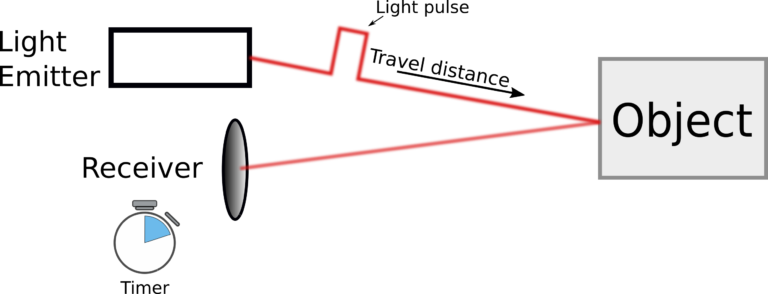
\includegraphics[width=\textwidth]{chapter03/img/tof_traveltime_original.png}
        \caption{One way to measure the time-of-flight for photons is to emit a light pulse and measure the roundtrip time until the reception of the reflection.}\label{fig:tof_roundtrip}
    \end{subfigure}\quad
    \begin{subfigure}[t]{0.45\textwidth}
        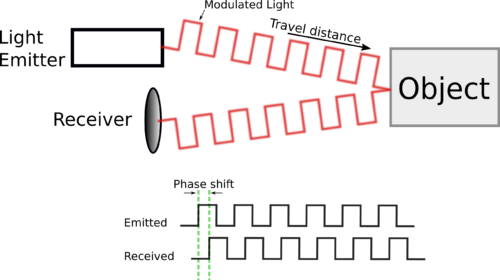
\includegraphics[width=\textwidth]{chapter03/img/tof_phase_shift_original.png}
        \caption{The second, more recent approach is measuring the phase-shift of photons relative to the light source. This allows a continously emitting light source.}\label{fig:tof_phase_shift}
    \end{subfigure}
    \caption[Illustration of the measuring principles for \acrshort{ToF} cameras]{\emph{Illustration of the measuring principles for \acrshort{ToF} cameras.} \acrlong{ToF} is first of all a measurement principle for distances used in different contexts. In this specific case \acrshort{ToF} sensors measure the roundtrip time of light from emittance, reflection and sensing. Multiplying the measured time by the speed of light results in the distance the light traveled. The illustrations are adopted from\cite{tof_cameras}.}\label{fig:tof_illustration}
\end{figure}

The second prevalent sensing technologies measure the traveling time of light.
Multiplying the measured roundtrip time by the known speed of light in the surrounding medium results in twice the distance of the object.
Such a sensor system requires a light sources, like structured light sensors.
Unlike the specialized patterns emitted for structured light, this can be an ordinary infrared LED, again preventing interference in other spectra of light.

A pulsed and synchronized light emitter, as examplarized in figure~\ref{fig:tof_roundtrip}, allows direct measurement of the roundtrip time of light.
Such a system requires exact synchronisation and a high temporal resolution to achieve accurate measurements.
The different, and more recent development in depth sensing technology, is measuring the phase shift (figure~\ref{fig:tof_phase_shift}) of the reflected light to recover the traveling time of the light wave.
This is the underlying principle of the Kinectv2 depth sensor.
The drawback of this technology is the limitted range of the depth sensor, due to the ambiguity of the wave signal.
Using modulation techniques to create a wave signal with more than one frequency increases the range of the sensor.

\subsubsection{\acrlong{LIDAR} (\acrshort{LIDAR})}

\acrlong{LIDAR} (\acrshort{LIDAR}) uses the same measurement principle as \acrshort{ToF}-cameras.
It determines the distance of an object using roundtrip time measurements.
The difference between \acrshort{LIDAR} and \acrshort{ToF}-Cameras is the usage of a \acrshort{laser} as light source and the overall setup of the sensor system.
The most common configurations use a horizontally rotating mirror that reflects the beam into the room.
For vertical coverage, the measurement head is rotated in total.
Each complete horizontal measurement is called a scan line.

Some \acrshort{LIDAR}s, especially mobile systems with real time requirements, measure in the order of magnitude $10^1$ number of scan lines.
Such systems achieve a higher framerate.
A dense \acrshort{LIDAR} scan is required for the choosen feature-based approach.
Such scans can be created with terrestrial \acrshort{LIDAR} stations, common in geodesic applications.
Additionally, the intensity of the reflected light beam might be obtained as second measurement channel.

Flash \acrshort{LIDAR} is a scannerless type of \acrshort{LIDAR} that does not require a rotating mirror or other mechanical system.
A flash \acrshort{LIDAR} uses the measurement principles described for \acrshort{ToF}-cameras and measures a dense range image in one shot.
% TODO cite 10.1109/SSIAI.2010.5483929
